\documentclass[UTF8,12pt]{ctexart}

\usepackage[a4paper,margin=2.2cm]{geometry}
\usepackage{amsmath,amssymb,bm}
\usepackage{graphicx}
\usepackage{booktabs}
\usepackage{array}
\usepackage{caption}
\usepackage{subcaption}
\usepackage{float}
\usepackage{xcolor}
\usepackage{hyperref}
\usepackage{enumitem}
\usepackage{fancyhdr}
\usepackage{titlesec}

\hypersetup{
  colorlinks=true,
  linkcolor=blue!55!black,
  citecolor=blue!55!black,
  urlcolor=blue!55!black
}

\graphicspath{{figures/}}

\definecolor{DeepBlue}{HTML}{17324D}
\definecolor{SoftBlue}{HTML}{245A7A}
\definecolor{PanelGray}{HTML}{F4F6F8}

\titleformat{\section}{\Large\bfseries\color{DeepBlue}}{\thesection}{0.8em}{}
\titleformat{\subsection}{\large\bfseries\color{SoftBlue}}{\thesubsection}{0.7em}{}

\pagestyle{fancy}
\fancyhf{}
\lhead{Core-Shell / PV-Active Shell EP}
\rhead{\thepage}
\renewcommand{\headrulewidth}{0.3pt}
\setlength{\headheight}{15pt}
\emergencystretch=2em

\setlength{\parindent}{2em}
\setlength{\parskip}{0.35em}
\setlist[itemize]{leftmargin=2.2em,itemsep=0.2em}
\captionsetup{font=small,labelfont=bf}

\newcommand{\dd}{\mathrm{d}}
\newcommand{\p}{\partial}
\newcommand{\avg}[1]{\left\langle #1 \right\rangle}
\newcommand{\core}{\mathcal{C}}
\newcommand{\shell}{\mathcal{S}}
\newcommand{\exchange}{\mathcal{E}}

\title{\textbf{Core-Shell / PV-Active Shell\\EP 分区理论说明}}
\author{S-H-I-T-ocean / Kuroshiou EP-FLUX 工作记录}
\date{2026-09-05}

\begin{document}
\maketitle

\begin{abstract}
我们当前不再把一个中尺度涡旋强行看成单一、封闭、同时负责 trapping、stirring、PV anomaly 和 EP forcing 的材料体。
现有诊断显示，Hua 弱速中心与 LAVD 旋转相干中心较接近，而 PV anomaly core 存在系统性偏离。
与此同时，热通量、PV 通量和 EP 倾斜修正并不都集中在低泄漏的 inner core 内，而是相当一部分出现在外侧 PV-active shell。
因此，本文提出并整理一个用于后续验证的双区结构：
\begin{equation}
\mathcal{T}_{total}
=
\mathcal{T}_{core}^{trap}
+
\mathcal{T}_{shell}^{stir}
+
\mathcal{T}_{exchange}.
\end{equation}
其中 inner core 负责 trapping/material coherence，PV-active shell 负责 heat/PV stirring 与 EP 倾斜修正的主要活跃区，exchange layer 负责两者之间的边界交换。
\end{abstract}

\section{为什么 single material eddy volume 不够用}

单一材料涡体积的理想假设是：存在一个边界 \(M\)，它既低泄漏，又包住弱速旋转中心，还包住主要 PV anomaly，并能让热、PV、动量输送都在内部闭合。
这个想法物理上很诱人，但我们的验证结果表明它过强。

第一，材料边界 leakage 不能忽略。
即使边界从阈值 mask 推进到 active/level-set/Lagrangian proxy，边界通量仍然不为零。
第二，thin curved tube 的小曲率前提失败。
该理论中的 metric/Jacobian/Christoffel 项需要
\begin{equation}
\epsilon_{\kappa}=\kappa r \ll 1,
\end{equation}
但我们的结果中 \(\epsilon_{\kappa}\) 中位数约为 \(10\sim 35\)，且 metric valid fraction 的中位数为 0。
第三，Hua/LAVD core 与 PV anomaly core 不共位。
LAVD 能找到旋转相干核，Hua 能找到弱速/速度几何中心，但 PV anomaly 最大区经常偏在 shell 或边界交换区。

所以，EP 闭合失败未必说明 EP 思路错误，更可能说明 ``一个边界同时圈住材料相干核与 PV 动力核'' 的对象设定本身不合适。

\begin{figure}[H]
  \centering
  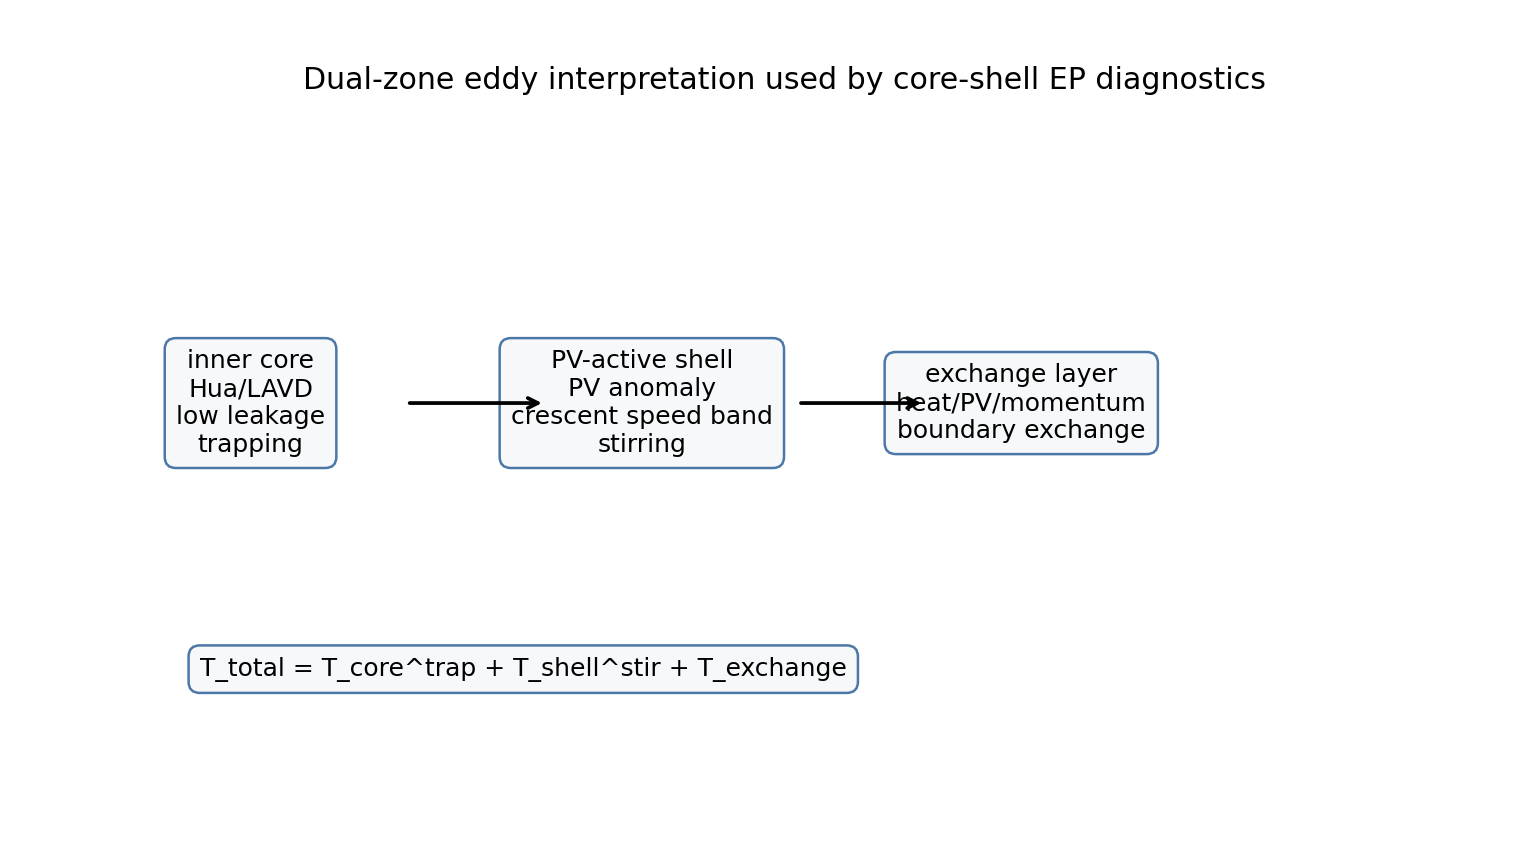
\includegraphics[width=0.82\linewidth]{dual_zone_framework_summary.png}
  \caption{双区结构框架：inner material core、PV-active shell 与 exchange layer 分账。该图给出当前理论模型的工作图像，而不是替代严格材料体理论。}
  \label{fig:dual-zone}
\end{figure}

\section{三类中心与核心}

\subsection{Hua 弱速中心}

Hua 中心来自速度场几何：局地速度异常低值、环向切向性、两侧反转和 boundary-monotonic 旋转约束。
它回答的是：这个位置是否像一个速度几何上的涡旋中心。
因此 Hua 中心偏运动学，适合描述弱速核、速度零线附近结构和可识别的旋转几何。

\subsection{LAVD 旋转相干中心}

LAVD 中心来自有限时间粒子轨迹上的涡度偏差积分 \cite{HallerEtAl2016}：
\begin{equation}
\mathrm{LAVD}_{t_0}^{t_1}(\bm{x}_0)
=
\int_{t_0}^{t_1}
\left|
\zeta(\bm{x}(t;\bm{x}_0),t)-\overline{\zeta}(t)
\right|
\dd t .
\end{equation}
它强调客观旋转相干性，适合定义材料旋转核。
但 LAVD 的高值区不必然等于 PV anomaly 的极值区。

\subsection{PV anomaly core}

PV anomaly core 是动力核心，表示 \(q'\) 或 PV proxy 的主要异常区。
若背景剪切、倾斜、密度结构或月牙状强速带显著，PV core 可以偏离弱速中心和 LAVD 中心。
这一分离是双区模型的起点：运动学旋转核不必等于动力 PV 核。

\section{Core-Shell-Exchange 分区模型}

我们定义三个区域：

\begin{itemize}
  \item \textbf{inner core}：围绕 Hua/LAVD 近同位中心的低 leakage 区域，主要物理意义是 trapping 与 material coherence。
  \item \textbf{PV-active shell}：围绕 inner core 的外壳，包含较强 PV anomaly、强剪切、非轴对称月牙状速度带，主要物理意义是 stirring、协方差输送和倾斜修正。
  \item \textbf{exchange layer}：inner core 与 PV-active shell 的界面。若界面上的热/PV/动量边界通量不小，就不能把 inner core 单独视作完整输送闭合体。
\end{itemize}

对应的总输送分解为
\begin{equation}
\mathcal{T}_{total}
=
\mathcal{T}_{core}^{trap}
+
\mathcal{T}_{shell}^{stir}
+
\mathcal{T}_{exchange}.
\end{equation}

这里的重点是：\(\mathcal{T}_{core}^{trap}\) 与 \(\mathcal{T}_{shell}^{stir}\) 是不同物理机制。
不能因为二者都属于 ``涡旋''，就用一个平均代表涡相乘来代替。

\section{热/PV stirring 必须用 aggregate-product}

热输送和 PV 输送必须使用乘积后平均，而不是平均后乘积。
对任一区域 \(M\)，定义
\begin{equation}
H_M^{stir}
=
\rho_0 C_p
\avg{v_{rot}'\theta'}_M ,
\end{equation}
\begin{equation}
P_M^{stir}
=
\avg{v_{rot}'q'}_M .
\end{equation}
同时保留失败对照：
\begin{equation}
\avg{vX}_M,\qquad
\avg{v}_M\avg{X}_M,\qquad
\mathrm{Cov}_M(v,X)
=
\avg{vX}_M
-
\avg{v}_M\avg{X}_M ,
\end{equation}
其中 \(X=\theta'\) 或 \(q'\)。
如果只用平均代表涡的 \(v\) 和 \(\theta/q\) 相乘，就会丢掉协方差输送。

\begin{figure}[H]
  \centering
  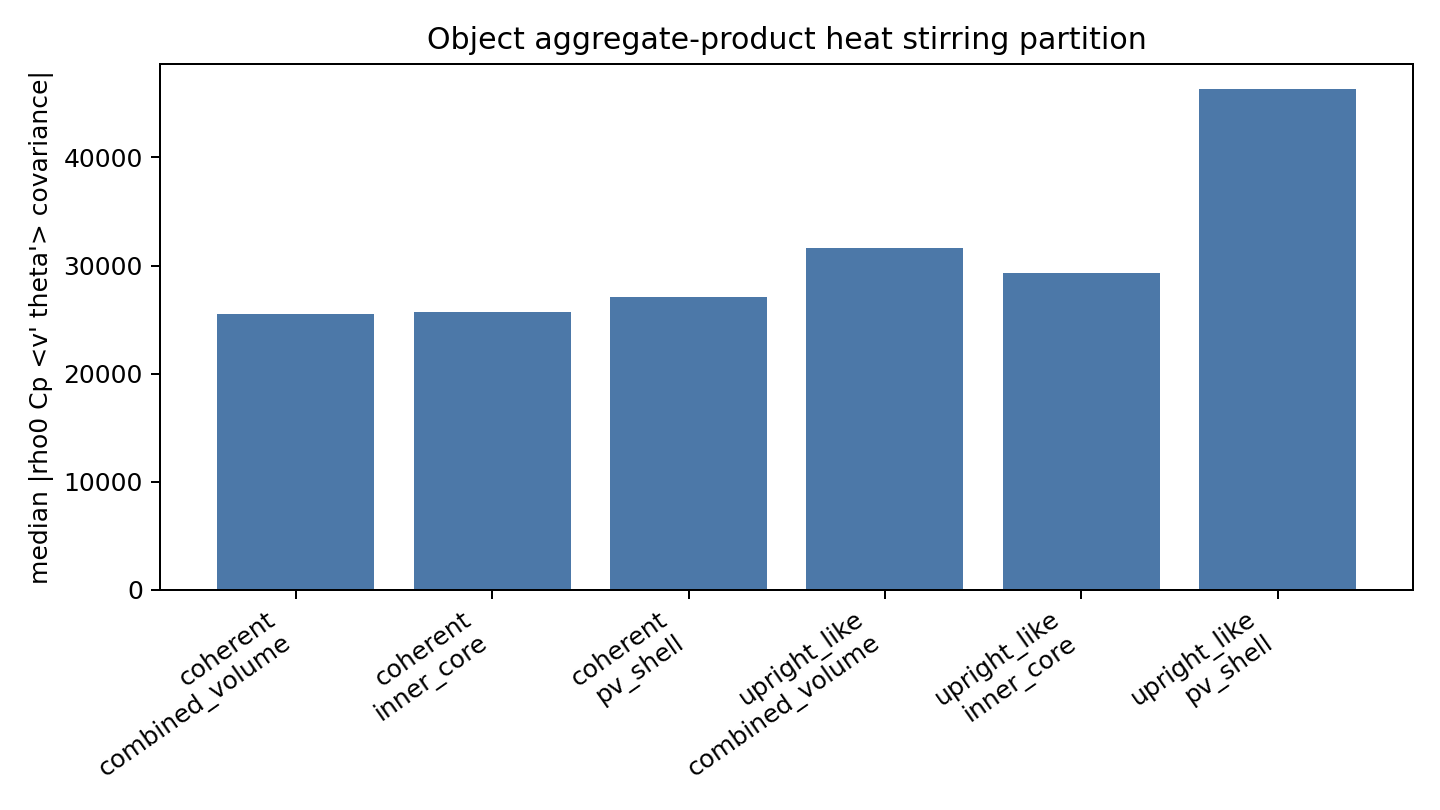
\includegraphics[width=0.88\linewidth]{object_aggregate_heat_core_vs_shell_partition.png}
  \caption{object-day aggregate-product 热通量分区。coherent 中 heat stirring 接近 core/shell 分担；upright\_like 中 shell 占比更高。}
  \label{fig:heat-partition}
\end{figure}

\begin{figure}[H]
  \centering
  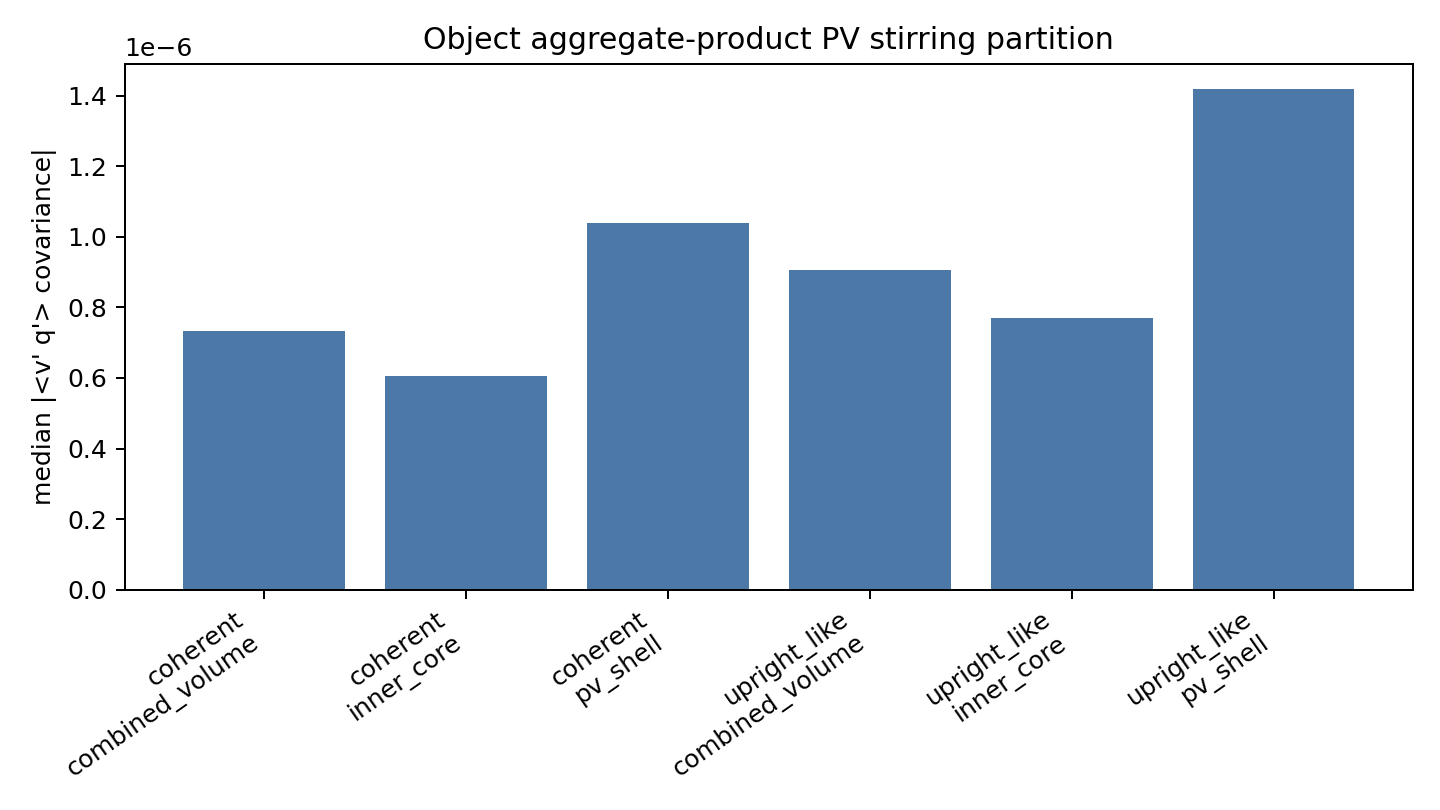
\includegraphics[width=0.88\linewidth]{object_aggregate_pv_core_vs_shell_partition.png}
  \caption{object-day aggregate-product PV 通量分区。PV covariance 更偏向 PV-active shell，说明 PV 动力输送并不主要由低泄漏 inner core 单独承担。}
  \label{fig:pv-partition}
\end{figure}

\section{普通垂向 EP flux 与倾斜坐标修正}

在局地轴向坐标中，把水平扰动速度分解为沿轴方向 \(u_s'\) 与法向方向 \(u_n'\)。
普通垂向 EP flux 可写为浮力通量项：
\begin{equation}
F_z^{ordinary}
=
\rho_0 f_0
\frac{\avg{u_n'b'}}{N^2}.
\end{equation}

当涡旋中心线倾斜时，真正沿倾斜涡旋坐标的垂向导数不等于欧拉固定 \(z\) 方向导数。
设中心线为 \(\bm{r}_c(z)\)，则
\begin{equation}
\partial_z^{tilted}
=
\partial_z
-
\frac{\dd \bm{r}_c}{\dd z}\cdot\nabla_h .
\end{equation}
因此可把倾斜坐标 EP flux 写成
\begin{equation}
F_z^{tilted}
=
F_z^{ordinary}
+
F_z^{tilt\ correction}.
\end{equation}

全生命周期 EP 验证显示
\begin{equation}
\mathrm{median}
\left(
\frac{|F_z^{tilt\ correction}|}{|F_z^{ordinary}|}
\right)
\approx 0.47,
\end{equation}
p25--p75 约为 0.32--0.62，最大可超过 1。
这说明倾斜修正不是小量；若用倾斜涡旋坐标，热/浮力相关的垂向 EP flux 会被明显改写。

\begin{figure}[H]
  \centering
  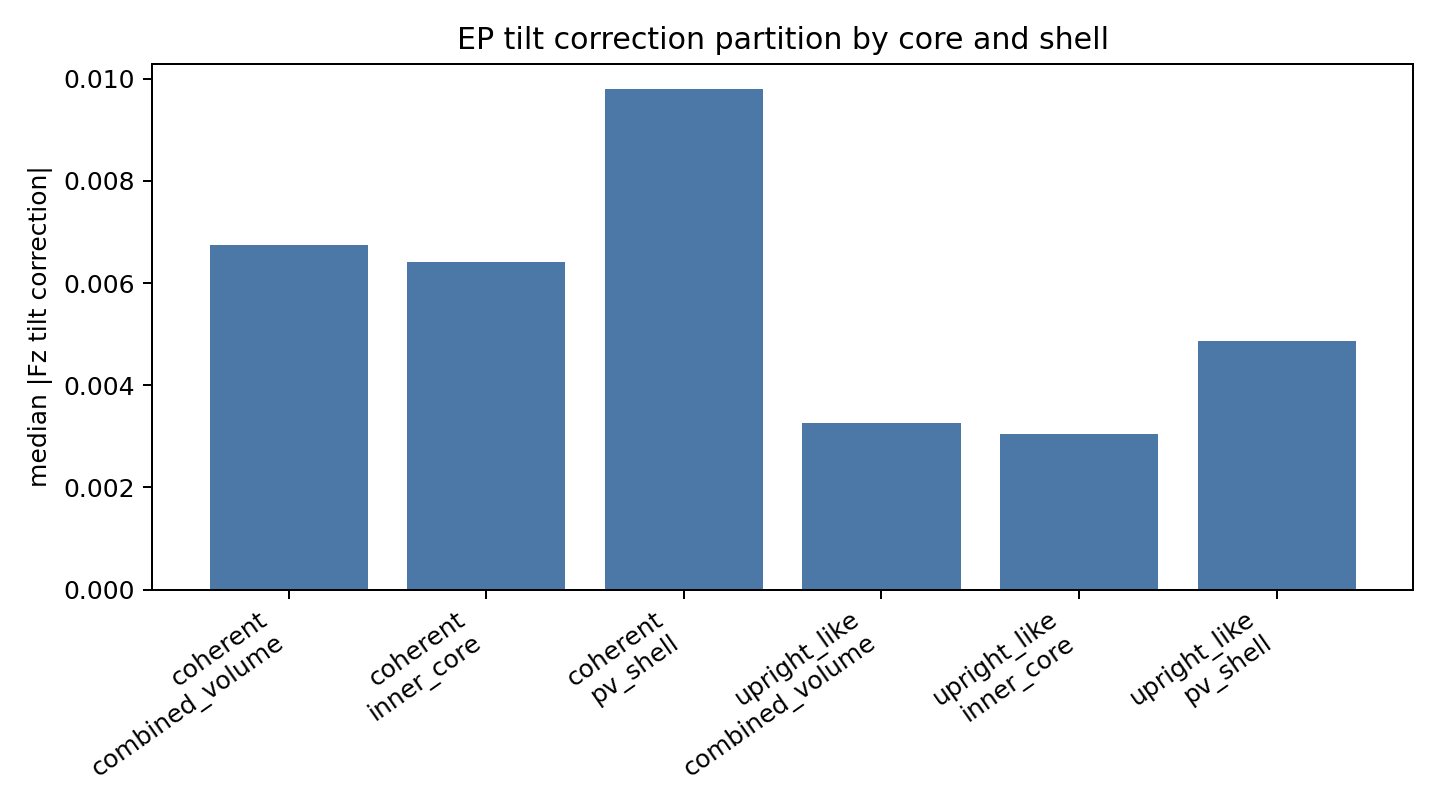
\includegraphics[width=0.88\linewidth]{ep_tilt_correction_core_vs_shell.png}
  \caption{EP 倾斜修正的 core-shell 分区。绝对贡献更偏 shell，说明 tilt correction 的主要信号并不只来自低泄漏材料核。}
  \label{fig:ep-tilt}
\end{figure}

\section{Exchange layer 与边界预算}

若 inner core 是严格材料体，边界法向通量应足够小。
但我们看到 core-shell interface 和总边界通量都不为零。
对热、PV、浮力和动量而言，这意味着边界交换不能被塞进单一 ``内部 EP forcing'' 里。

边界预算应单独写为：
\begin{align}
\mathcal{B}_{heat}
&=
\oint_{\partial M}
\rho_0 C_p \theta' u_n\,\dd S,\\
\mathcal{B}_{PV}
&=
\oint_{\partial M}
q' u_n\,\dd S,\\
\mathcal{B}_{mom,i}
&=
\oint_{\partial M}
u_i' u_n\,\dd S .
\end{align}

闭合残差应被理解为
\begin{equation}
R_{closure}
=
\left|
\mathcal{F}_{interior}^{EP}
+
\mathcal{B}_{exchange}
\right| .
\end{equation}
如果 \(R_{closure}\) 不下降，不能简单调边界到 ``看起来更封闭''；
更可能说明 PV-active shell 和 inner material core 是两个不同物理区。

\begin{figure}[H]
  \centering
  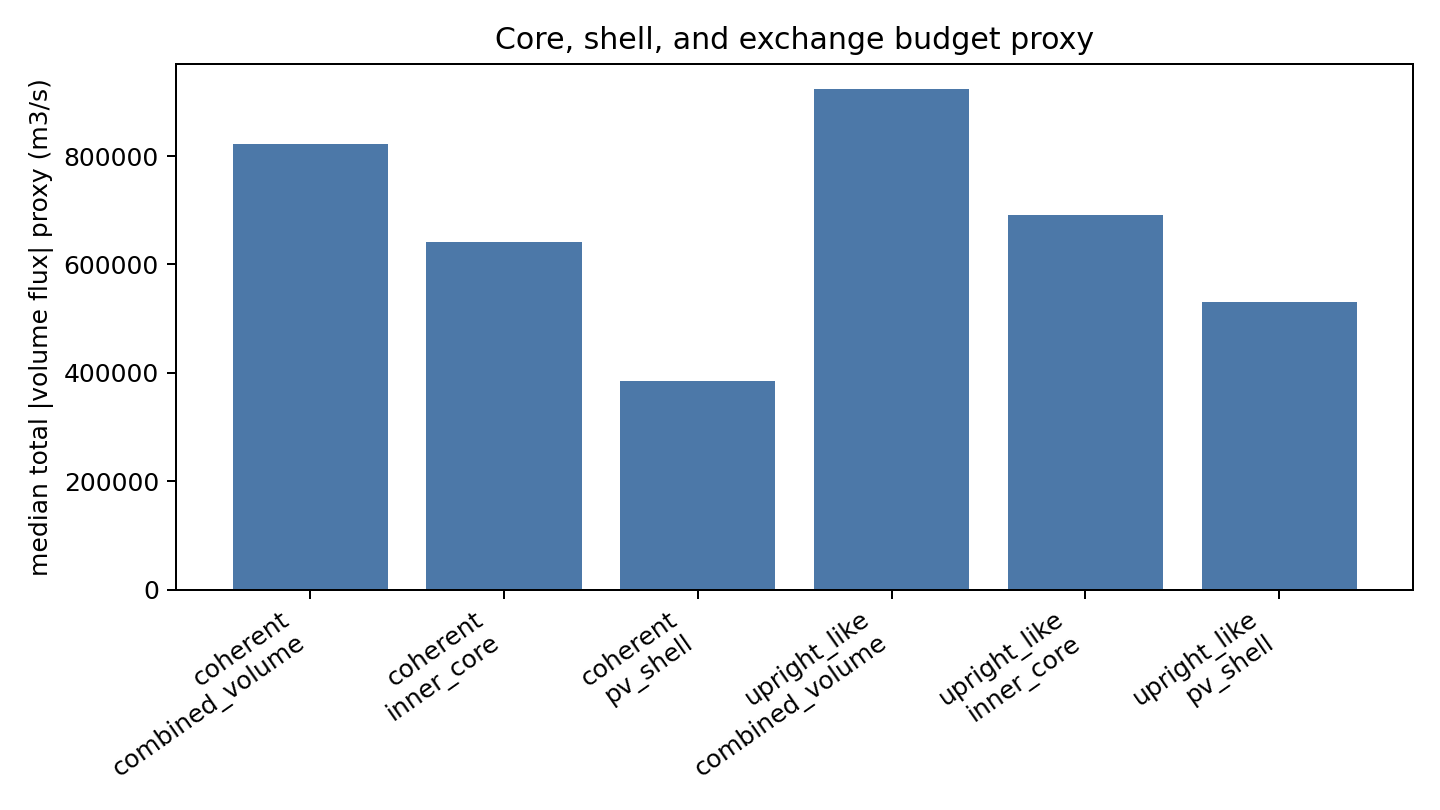
\includegraphics[width=0.88\linewidth]{core_shell_exchange_budget.png}
  \caption{core-shell exchange budget。低 leakage core 可以用于 trapping 解释，但不能自动代表全部热/PV/动量输送。}
  \label{fig:exchange}
\end{figure}

\begin{figure}[H]
  \centering
  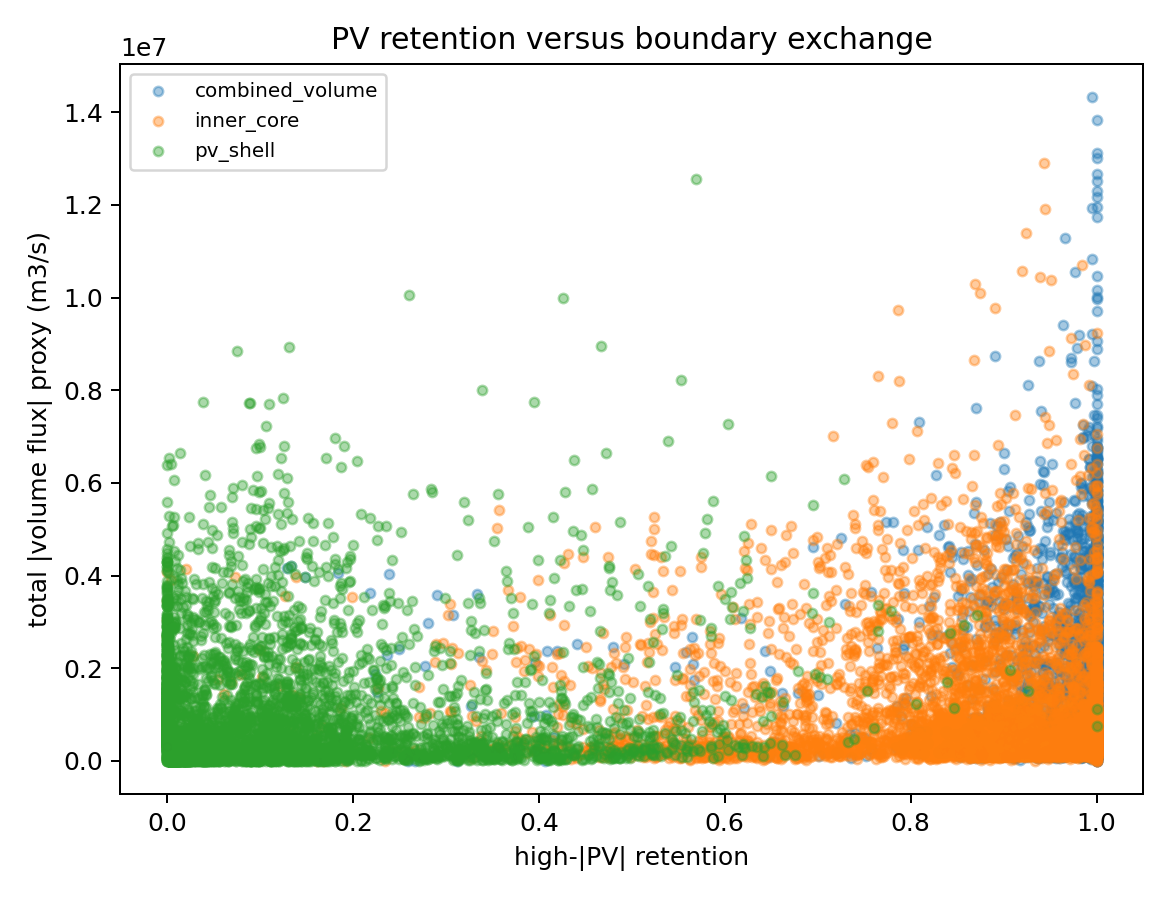
\includegraphics[width=0.88\linewidth]{pv_retention_vs_boundary_exchange.png}
  \caption{PV retention 与 boundary exchange 的关系。若提高 PV retention 的同时 leakage 或 exchange 增大，则支持 ``PV 动力核不完全属于低泄漏旋转材料核'' 的解释。}
  \label{fig:pv-retention}
\end{figure}

\section{与前人工作的关系}

Haller 与 Beron-Vera 的 geodesic eddy 理论强调有限时间低拉伸的闭合材料边界 \cite{HallerBeronVera2013}；
Haller 等人的 LAVD 理论强调客观旋转相干核 \cite{HallerEtAl2016}。
这两类方法都很适合定义 inner material core，但它们并不要求 PV anomaly core 必须被同一个边界完全包住。

Abernathey 与 Haller 对 eastern Pacific 的研究提醒：Eulerian eddy 与 Lagrangian coherent vortex 并不等价，许多表观涡输送会被 filamentation 和 leakage 削弱 \cite{AbernatheyHaller2018}。
这个结论与我们现在的 exchange layer 解释一致。

Hausmann 与 Czaja、Dong 等关于 eddy heat transport 的工作说明，热输送本质上来自速度与温度异常的协方差 \cite{HausmannCzaja2012,DongEtAl2014}。
Chelton 等和 Frenger 等给出的全球/南大洋涡旋统计，则说明 ``涡旋结构'' 和 ``涡旋输送'' 不能混为一个量 \cite{CheltonEtAl2011,FrengerEtAl2015}。
Greatbatch 的 EP/PV flux 关系则为把动量、浮力与 PV 通量放到同一预算中提供了动力学背景 \cite{Greatbatch1998}。

Yang/Xu/Li 2026 的模态分解工作说明，垂向倾斜可以由第一、第二斜压模态传播差异产生 \cite{YangXuLi2026Local}。
我们的结果进一步指出：在 Kuroshiou 的速度中心和代表涡框架下，倾斜修正会明显改写 EP 垂向通量；
但由于 PV core 与旋转材料核分离，不能直接用单一材料体闭合来解释全部 PV/热输送。

\section{当前判定}

\begin{table}[H]
\centering
\caption{当前理论判定摘要}
\begin{tabular}{p{4.0cm}p{8.6cm}p{2.1cm}}
\toprule
问题 & 当前判定 & 证据等级\\
\midrule
倾斜修正是否重要 & \(|F_z^{tilt\ correction}|/|F_z^{ordinary}|\) 中位数约 0.47 & 强\\
thin curved tube 是否可强解释 & metric valid fraction 中位数为 0；\(\kappa r\) 约 10--35 & 否\\
热/PV stirring 来自哪里 & PV 与 EP tilt 更偏 shell；heat 在 coherent 中近分担 & 中-强\\
PV core 是否必须在 LAVD core 内 & 不应强制；二者可系统性分离 & 中\\
推荐理论框架 & core trap + shell stir + exchange & 当前最佳\\
\bottomrule
\end{tabular}
\end{table}

当前最稳健的正结果是：倾斜坐标修正不是小量，约为 ordinary vertical EP flux 的一半量级。
最需要谨慎的部分是：曲管 metric/Jacobian/Christoffel 项不能强解释，因为小曲率条件失败。
最有解释力的新方向是：把材料相干核、PV-active shell 和 exchange layer 分开，而不是继续强行要求 \(PV\ core \subset M_{LAVD}\)。

\section{后续验证路线}

下一步应围绕三件事继续。
第一，在 object-level 上验证 particle retention、LAVD/geodesic boundary 和 leakage，而不是把代表涡平均场当成严格材料体。
第二，在 PV-active shell 中继续做 aggregate-product heat/PV/momentum moments，确认 shell 是否稳定承载主要 stirring。
第三，把 exchange layer 的 boundary heat/PV/momentum flux 与 interior EP forcing 分账，判断闭合残差来自边界交换、PV proxy、浮力口径，还是缺失三维通量项。

如果这些验证成立，后续论文叙述应从 ``一个倾斜材料涡旋的 EP 闭合'' 改成：
``倾斜涡旋的材料核、PV-active 外壳与交换层共同决定热/PV/动量输送''。

\begin{thebibliography}{99}
\bibitem{HallerBeronVera2013}
Haller, G. and Beron-Vera, F. J. (2013).
Coherent Lagrangian vortices: the black holes of turbulence.
\textit{Journal of Fluid Mechanics}, 731, R4.
DOI: \href{https://doi.org/10.1017/jfm.2013.391}{10.1017/jfm.2013.391}.

\bibitem{HallerEtAl2016}
Haller, G., Hadjighasem, A., Farazmand, M., and Huhn, F. (2016).
Defining coherent vortices objectively from the vorticity.
\textit{Journal of Fluid Mechanics}, 795, 136--173.
DOI: \href{https://doi.org/10.1017/jfm.2016.151}{10.1017/jfm.2016.151}.

\bibitem{AbernatheyHaller2018}
Abernathey, R. and Haller, G. (2018).
Transport by Lagrangian Vortices in the Eastern Pacific.
\textit{Journal of Physical Oceanography}, 48, 667--685.
DOI: \href{https://doi.org/10.1175/JPO-D-17-0102.1}{10.1175/JPO-D-17-0102.1}.

\bibitem{CheltonEtAl2011}
Chelton, D. B., Schlax, M. G., and Samelson, R. M. (2011).
Global observations of nonlinear mesoscale eddies.
\textit{Progress in Oceanography}, 91, 167--216.
DOI: \href{https://doi.org/10.1016/j.pocean.2011.01.002}{10.1016/j.pocean.2011.01.002}.

\bibitem{HausmannCzaja2012}
Hausmann, U. and Czaja, A. (2012).
The observed signature of mesoscale eddies in sea surface temperature and the associated heat transport.
\textit{Nature Communications}, 3, 884.
DOI: \href{https://doi.org/10.1038/ncomms1595}{10.1038/ncomms1595}.

\bibitem{DongEtAl2014}
Dong, C., Zhang, Y., Gille, S. T., et al. (2014).
Global estimates of oceanic mesoscale eddy heat and salt transports from Argo and altimetry.
\textit{Nature Communications}, 5, 3294.
DOI: \href{https://doi.org/10.1038/ncomms4294}{10.1038/ncomms4294}.

\bibitem{FrengerEtAl2015}
Frenger, I., Munnich, M., Gruber, N., and Knutti, R. (2015).
Southern Ocean eddy phenomenology.
\textit{Journal of Geophysical Research: Oceans}, 120, 7413--7449.
DOI: \href{https://doi.org/10.1002/2015JC011047}{10.1002/2015JC011047}.

\bibitem{Greatbatch1998}
Greatbatch, R. J. (1998).
Exploring the relationship between eddy-induced transport velocity, vertical momentum transfer, and the isopycnal flux of potential vorticity.
\textit{Journal of Physical Oceanography}, 28, 422--432.
DOI: \href{https://doi.org/10.1175/1520-0485(1998)028<0422:ETRBEI>2.0.CO;2}{10.1175/1520-0485(1998)028<0422:ETRBEI>2.0.CO;2}.

\bibitem{YangXuLi2026Local}
Yang, Z., Xu, F., and Li, H. (2026).
Understanding the Mesoscale Eddy Vertical Tilt Based on Mode Decomposition.
Local PDF: \texttt{C:/Users/chenz/Desktop/PAPER/2026\_Li\_...Tilt\_Bas.pdf}.

\bibitem{InternalEPNotes}
Project internal notes:
\textit{E-P\_flux理论整理.pdf};
\textit{curved\_tube\_ep\_flux.pdf};
\textit{large\_curvature\_material\_volume\_ep\_flux.pdf}.
\end{thebibliography}

\end{document}
